\chapter{Résultats}
Dans cette partie, nous allons tout d'abord analyser les tests effectués sur des données de synthèse pour valider l'implémentation de FABEMD. Ensuite, nous verrons les résultats obtenus sur des données réelles.
\section{Validation sur données de synthèse}
Pour valider l'implémentation faite de l'algorithme FABEMD, nous allons tout d'abord analyser les résultats produits sur des données de synthèse. Pour ce faire, nous allons générer des images composées de sinusoïdes (figure \ref{fig:s}) et nous chercherons à extraire celles-ci dans chaque BIMF produit par FABEMD. Nous effectuerons nos tests en faisant varier deux des paramètres ayant une influence sur les décompositions produites : le choix de la taille des filtres et le nombre maximal d'itérations pour la génération d'un BIMF.
On peut observer qu'on obtient des résultats similaires aux résultats obtenus dans l'article. Le type 4 (figures \ref{fig:s_1_4} et \ref{fig:s_5_4}) de taille de filtre permet d'obtenir des résultats en un nombre d'itérations moins important. De même, comme décrit par Bhuiyan et al., les résultats obtenus par FABEMD sont optimaux lorsque l'on utilise un nombre maximal d'itérations égal à 1 (figures \ref{fig:s_1_1} et \ref{fig:s_1_4}). Par la suite, on favorisera donc ce paramètre pour l'utilisation de FABEMD sur des données réelles.

\begin{figure}
\centering
\begin{subfigure}{.30\textwidth}
  \centering
  
\includegraphics[width=.9\linewidth]{img/s_0}
  \caption{Composante 1}
\end{subfigure}
\begin{subfigure}{.30\textwidth}
  \centering
  
\includegraphics[width=.9\linewidth]{img/s_1}
  \caption{Composante 2}
\end{subfigure}
\begin{subfigure}{.30\textwidth}
  \centering
  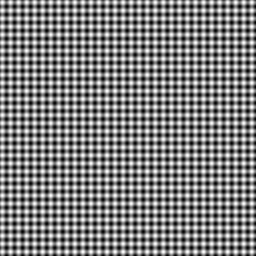
\includegraphics[width=.9\linewidth]{img/s_2}
  \caption{Composante 3}
\end{subfigure}
\begin{subfigure}{.30\textwidth}
  \centering
  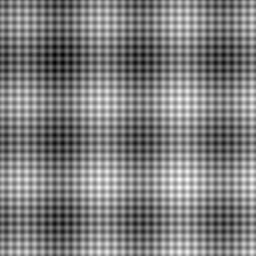
\includegraphics[width=.9\linewidth]{img/s_c}
  \caption{Somme des composantes}
\end{subfigure}
\caption{Image de synthèse et composantes utilisées pour les tests}
\label{fig:s_1_4}
\end{figure}

\begin{figure}
\centering
\begin{subfigure}{.30\textwidth}
  \centering
  
\includegraphics[width=.9\linewidth]{img/s_1_1_1}
  \caption{BIMF 1}
\end{subfigure}
\begin{subfigure}{.30\textwidth}
  \centering
  
\includegraphics[width=.9\linewidth]{img/s_1_1_2}
  \caption{BIMF 2}
\end{subfigure}
\begin{subfigure}{.30\textwidth}
  \centering
  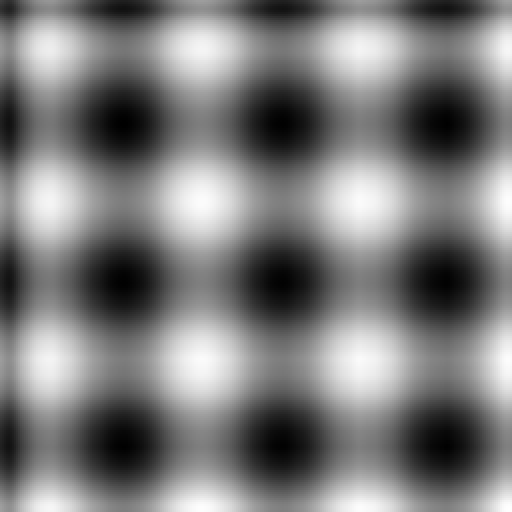
\includegraphics[width=.9\linewidth]{img/s_1_1_3}
  \caption{BIMF 3}
\end{subfigure}
\begin{subfigure}{.30\textwidth}
  \centering
  
\includegraphics[width=.9\linewidth]{img/s_1_1_4}
  \caption{BIMF 4}
\end{subfigure}
\begin{subfigure}{.30\textwidth}
  \centering
  
\includegraphics[width=.9\linewidth]{img/s_1_1_5}
  \caption{BIMF 5}
\end{subfigure}
\begin{subfigure}{.30\textwidth}
  \centering
  
\includegraphics[width=.9\linewidth]{img/s_1_1_6}
  \caption{BIMF 6}
\end{subfigure}
\caption{Résultats obtenus avec FABEMD en utilisant au maximum 1 itération et une taille de filtre de type 1}
\label{fig:s_1_1}
\end{figure}

\begin{figure}
\centering
\begin{subfigure}{.30\textwidth}
  \centering
  
\includegraphics[width=.9\linewidth]{img/s_1_4_1}
  \caption{BIMF 1}
\end{subfigure}
\begin{subfigure}{.30\textwidth}
  \centering
  
\includegraphics[width=.9\linewidth]{img/s_1_4_2}
  \caption{BIMF 2}
\end{subfigure}
\begin{subfigure}{.30\textwidth}
  \centering
  
\includegraphics[width=.9\linewidth]{img/s_1_4_3}
  \caption{BIMF 3}
\end{subfigure}
\caption{Résultats obtenus avec FABEMD en utilisant au maximum 1 itération et une taille de filtre de type 4}
\label{fig:s_1_4}
\end{figure}

\begin{figure}
\centering
\begin{subfigure}{.30\textwidth}
  \centering
  
\includegraphics[width=.9\linewidth]{img/s_5_1_1}
  \caption{BIMF 1}
\end{subfigure}
\begin{subfigure}{.30\textwidth}
  \centering
  
\includegraphics[width=.9\linewidth]{img/s_5_1_2}
  \caption{BIMF 2}
\end{subfigure}
\begin{subfigure}{.30\textwidth}
  \centering
  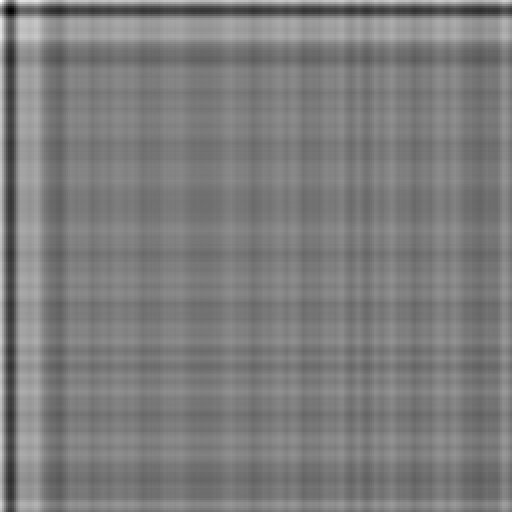
\includegraphics[width=.9\linewidth]{img/s_5_1_3}
  \caption{BIMF 3}
\end{subfigure}
\begin{subfigure}{.30\textwidth}
  \centering
  
\includegraphics[width=.9\linewidth]{img/s_5_1_4}
  \caption{BIMF 4}
\end{subfigure}
\begin{subfigure}{.30\textwidth}
  \centering
  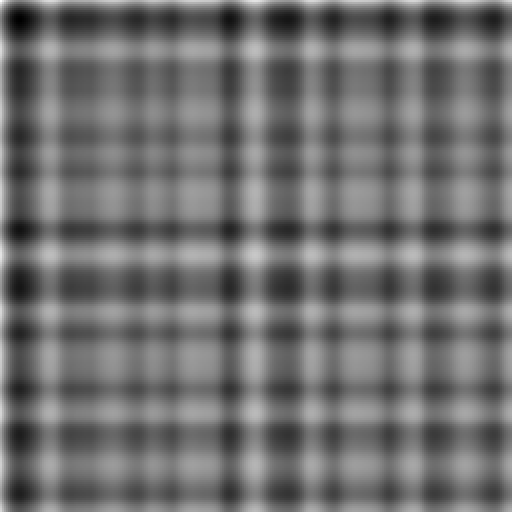
\includegraphics[width=.9\linewidth]{img/s_5_1_5}
  \caption{BIMF 5}
\end{subfigure}
\begin{subfigure}{.30\textwidth}
  \centering
  
\includegraphics[width=.9\linewidth]{img/s_5_1_6}
  \caption{BIMF 6}
\end{subfigure}
\begin{subfigure}{.30\textwidth}
  \centering
  
\includegraphics[width=.9\linewidth]{img/s_5_1_7}
  \caption{BIMF 7}
\end{subfigure}
\caption{Résultats obtenus avec FABEMD en utilisant au maximum 5 itérations et une taille de filtre de type 1}
\label{fig:s_5_1}
\end{figure}

\begin{figure}
\centering
\begin{subfigure}{.30\textwidth}
  \centering
  
\includegraphics[width=.9\linewidth]{img/s_5_4_1}
  \caption{BIMF 1}
\end{subfigure}
\begin{subfigure}{.30\textwidth}
  \centering
  
\includegraphics[width=.9\linewidth]{img/s_5_4_2}
  \caption{BIMF 2}
\end{subfigure}
\begin{subfigure}{.30\textwidth}
  \centering
  
\includegraphics[width=.9\linewidth]{img/s_5_4_3}
  \caption{BIMF 3}
\end{subfigure}
\caption{Résultats obtenus avec FABEMD en utilisant au maximum 5 itérations et une taille de filtre de type 4}
\label{fig:s_5_4}
\end{figure}

\section{Données réelles}

L'implémentation faite de FABEMD permet d'obtenir rapidement des décompositions correctes en fonctions modales intrinsèques. Nous pouvons désormais tester notre application sur des images réelles. Ici, nous utiliserons au maximum une itération pour la génération du BIMF et nous testerons avec les types de fenêtre de filtre 1 et 4. L'image de test utilisée sera celle utilisée dans l'article de recherche.

\begin{figure}
\centering
\begin{subfigure}{.30\textwidth}
  \centering
  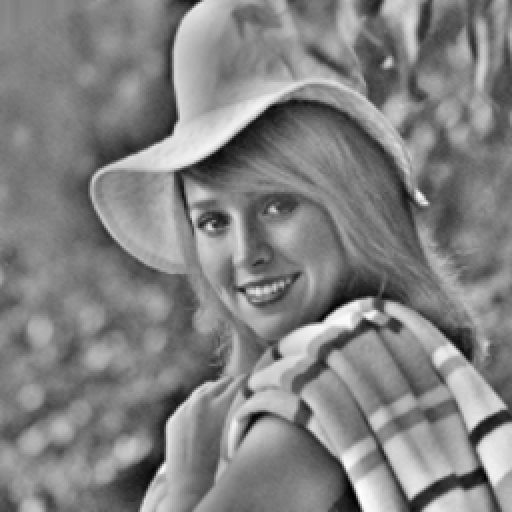
\includegraphics[width=.9\linewidth]{img/e_1_4_1}
  \caption{BIMF 1}
\end{subfigure}
\begin{subfigure}{.30\textwidth}
  \centering
  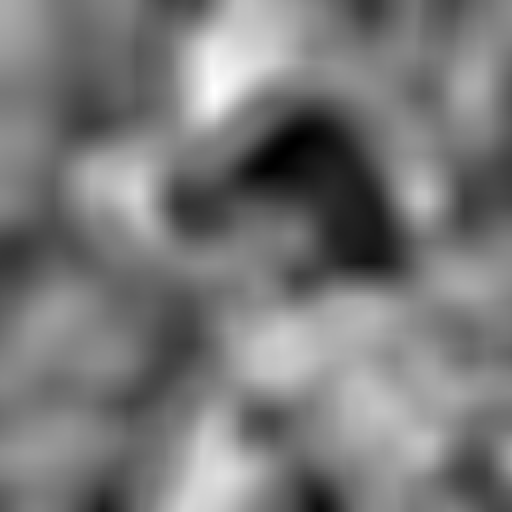
\includegraphics[width=.9\linewidth]{img/e_1_4_2}
  \caption{BIMF 2}
\end{subfigure}
\begin{subfigure}{.30\textwidth}
  \centering
  
\includegraphics[width=.9\linewidth]{img/e_1_4_3}
  \caption{BIMF 3}
\end{subfigure}
\begin{subfigure}{.30\textwidth}
  \centering
  
\includegraphics[width=.9\linewidth]{img/e_1_4_4}
  \caption{BIMF 4}
\end{subfigure}
\caption{Résultats obtenus avec FABEMD en utilisant au maximum 1 itérations et une taille de filtre de type 4 sur l'image d'Elaine}
\label{fig:e_1_4}
\end{figure}

\begin{figure}
\centering
\begin{subfigure}{.30\textwidth}
  \centering
  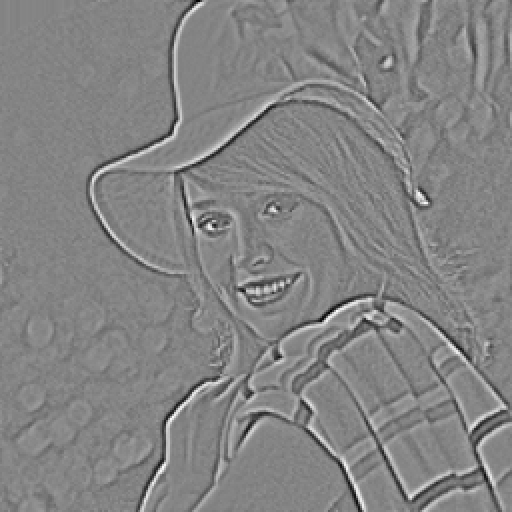
\includegraphics[width=.9\linewidth]{img/e_1_1_1}
  \caption{BIMF 1}
\end{subfigure}
\begin{subfigure}{.30\textwidth}
  \centering
  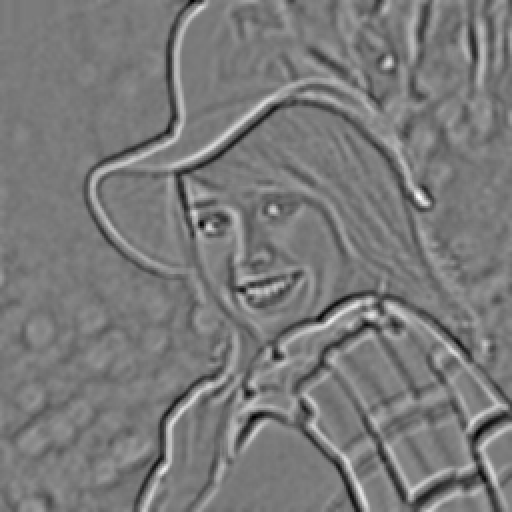
\includegraphics[width=.9\linewidth]{img/e_1_1_2}
  \caption{BIMF 2}
\end{subfigure}
\begin{subfigure}{.30\textwidth}
  \centering
  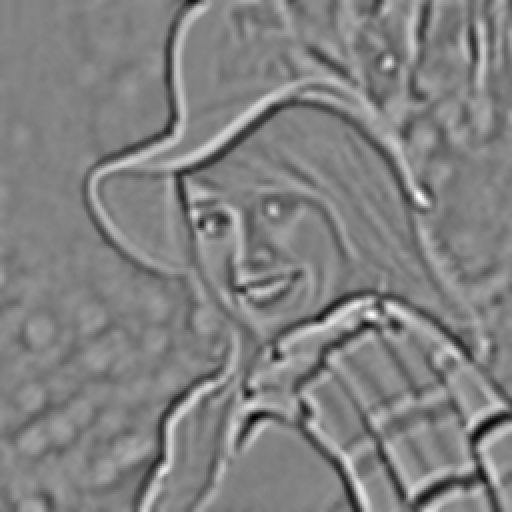
\includegraphics[width=.9\linewidth]{img/e_1_1_3}
  \caption{BIMF 3}
\end{subfigure}
\begin{subfigure}{.30\textwidth}
  \centering
  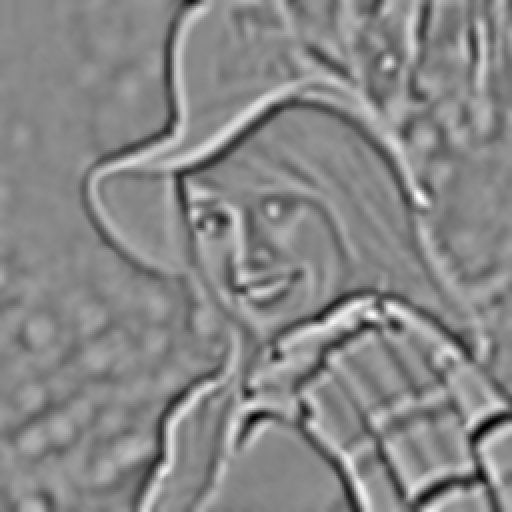
\includegraphics[width=.9\linewidth]{img/e_1_1_4}
  \caption{BIMF 4}
\end{subfigure}
\begin{subfigure}{.30\textwidth}
  \centering
  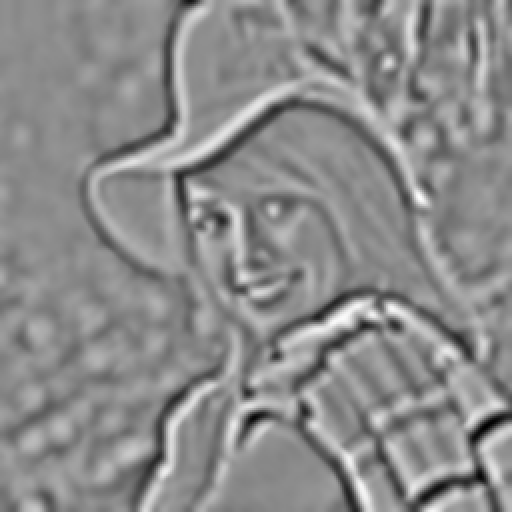
\includegraphics[width=.9\linewidth]{img/e_1_1_5}
  \caption{BIMF 5}
\end{subfigure}
\begin{subfigure}{.30\textwidth}
  \centering
  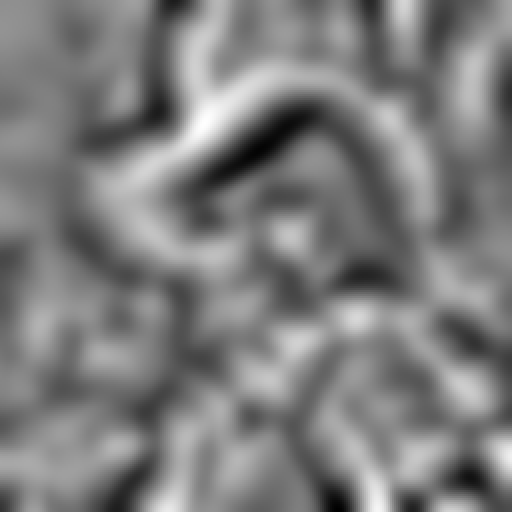
\includegraphics[width=.9\linewidth]{img/e_1_1_20}
  \caption{BIMF 20}
\end{subfigure}
\begin{subfigure}{.30\textwidth}
  \centering
  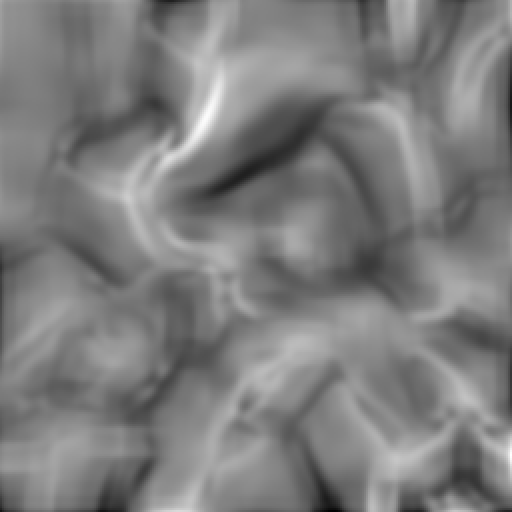
\includegraphics[width=.9\linewidth]{img/e_1_1_21}
  \caption{BIMF 21}
\end{subfigure}
\begin{subfigure}{.30\textwidth}
  \centering
  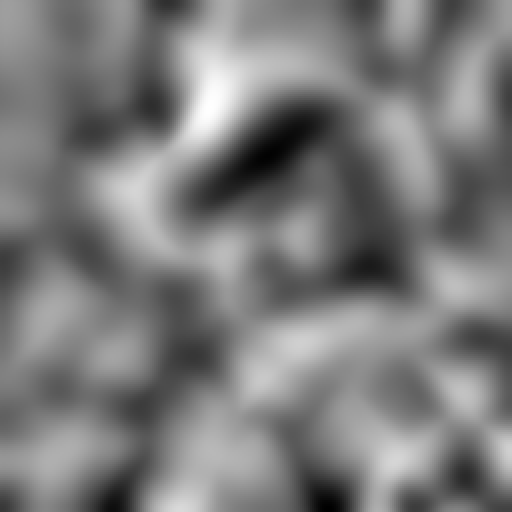
\includegraphics[width=.9\linewidth]{img/e_1_1_22}
  \caption{BIMF 22}
\end{subfigure}
\begin{subfigure}{.30\textwidth}
  \centering
  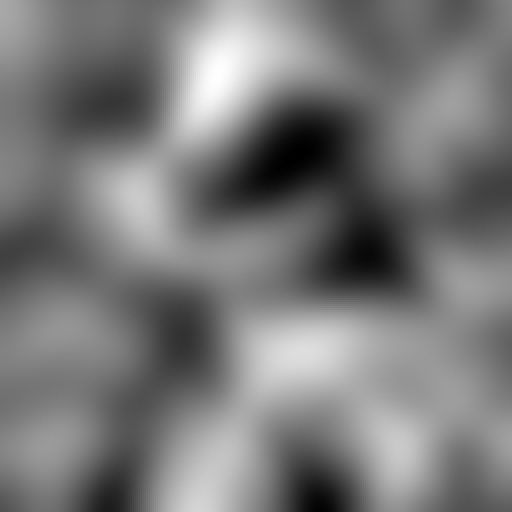
\includegraphics[width=.9\linewidth]{img/e_1_1_23}
  \caption{BIMF 23}
\end{subfigure}
\begin{subfigure}{.30\textwidth}
  \centering
  
\includegraphics[width=.9\linewidth]{img/e_1_1_24}
  \caption{BIMF 24}
\end{subfigure}
\begin{subfigure}{.30\textwidth}
  \centering
  
\includegraphics[width=.9\linewidth]{img/e_1_1_25}
  \caption{BIMF 25}
\end{subfigure}
\caption{Résultats obtenus avec FABEMD en utilisant au maximum 1 itérations et une taille de filtre de type 1 sur l'image d'Elaine}
\label{fig:e_5_4}
\end{figure}

